\documentclass[preview]{standalone}

\usepackage{amsmath,amsfonts,amsthm}
\usepackage[english]{babel} 
\usepackage[hscale=0.7,vscale=0.8]{geometry}
\usepackage[square,numbers]{natbib}

\usepackage{graphicx}
\usepackage{subcaption}
\usepackage{tikz}

\usetikzlibrary{shapes.misc, positioning}
\usetikzlibrary{fit,positioning}
\usetikzlibrary{bayesnet}

\begin{document}

\begin{figure}
	\centering
	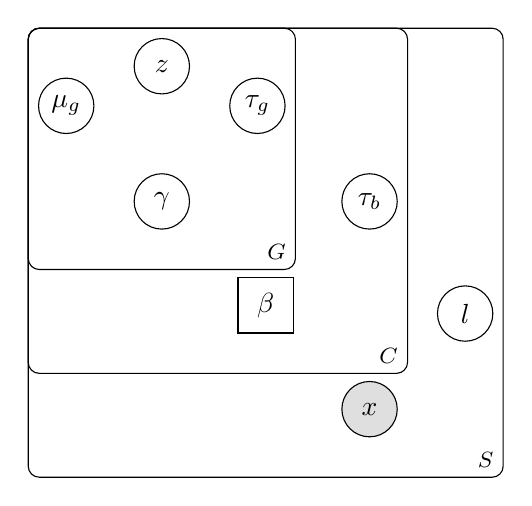
\begin{tikzpicture}
	\node[obs] (x) {$x$};
	\node[latent, above right = of x] (l) {$l$};
	\node[latent, rectangle, above left = of x] (beta) {$\beta$};
	\node[latent, above right = of beta] (taub) {$\tau_{b}$};
	\node[latent, above left = of beta] (gamma) {$\gamma$};
	\node[latent, above right = of gamma] (taug) {$\tau_g$};
	\node[latent, above = of gamma] (cat) {$z$};
	\node[latent, above left = of gamma] (mug) {$\mu_g$};

	\plate  {name} {(gamma)(taug)(cat)(mug)} {$G$};
	\plate  {name} {(gamma)(taug)(cat)(mug)(beta)(taub)} {$C$};
	\plate  {name} {(gamma)(taug)(cat)(mug)(beta)(taub)(l)(x)} {$S$};

	\end{tikzpicture}

\end{figure}
\end{document}





